\section{Methods}
We start with a description of `single locus multiple-time point'
models in which each locus is analyzed independently for evidence of a
selection constraint. In the subsequent section, we extend the
methodology to `linked-loci, multiple time' models where we consider
all linked loci within a small recombination-free window.

\subsection{Dynamics of the Sweep}

\subsection{Single-Locus Methods}
Consider a bi-allelic single-locus (Wright-Fisher like) model with no
mutations \cite{Ewens2012}, discrete generations, random mating
etc. With finite population size, the allele frequencies from
generation to generation are described by the random process
$\{x_{\ell,t}\}$ which denotes the population allele frequency at
locus $\ell$ at time generation $t$. The model has access to finite
number of observations in time for each locus, where the sampling
times are given by the set $\Tc=\{\tau_1,\tau_2,\cdots, \tau_T \}$
such that $\tau_1<\tau_2,\cdots<\tau_T$. We also assume that
measurements are taken up for $R$ experimental replicates for $L$
loci. Thus, The allele frequencies of a population are given by the
tensor $\bfX \in [0,1]^{R \times L \times T}$, where $X_{r,\ell,t}$
stores the observed of allele frequency at replicate $r$, locus $\ell$
and generation $\tau_t$. However, we often omit $r$ for clarity of
exposition. A neutrally evolving allele `drifts', and for a finite
population,
\beq x_{t+1} = x_t + \epsilon_t\; .\footnote{With infinite population size
  we have $x_{t+1} = x_t$, a restatement of Hardy-Weinberg
  equilibrium.}
\label{eq:drift}
\eeq where $\epsilon_t \sim \Nc(0,1)$ is a change due to genetic drift
in generation $t$.

\paragraph{Allele frequencies under selection.}
Consider next, a locus under selection with coefficient $s (0\le s\le
1)$, overdominance and parameter $h (0\le h\le 1)$, so that the
probability of an individual inheriting $2$ favored alleles is
$\propto (1+s)$, relative to inheriting $0$ favored
alleles. Respectively, the probability of favoring $1$ favored allele
$\propto (1+hs)$ Then,


\begin{equation}
x_{t+1} = f(x_t;s,h) + \epsilon_t
\label{eq:trans0} 
\end{equation}
where $f: [0,1] \mapsto [0,1]$ is the
transition function given by:
\begin{equation}
f(x;s,h)=\frac{(1+s)x^2 + (1+hs)x(1-x)}{(1+s)x^2 + 2(1+hs)x(1-x) + (1-x)^2}
    =x+\frac{s(h+(1-2h)x)x(1-x)}{1+sx(2h+(1-2h)x))}\;.
\end{equation}
We simplify notation by setting $h=0.5$, so that
\begin{equation}
  f(x;s,0.5)=x+\frac{sx(1-x)}{2+2sx}\;.
  \label{eq:hequalshalf}
\end{equation}
Our goal is to estimate $s$ given allele frequencies, and/or to decide
if $s>0$. Note that the dependence on $s$ is non-linear. Define an
auxiliary continuous (in time) function $\nu_t(s)$ as follows:
$\nu_0(s)=x_0$ for all $s$, and:
\begin{eqnarray}
  \nu_{t+\delta t}(s) &=& \nu_t(s)+\frac{\nu_t(s)(1-\nu_t(s))s\delta t}{2+2s\delta t \nu_t(s)}\;,\\
  \frac{d\nu_t(s)}{dt} &=&\lim_{\delta t\rightarrow 0}\frac{\nu_{t+\delta t}(s) -\nu_t(s)}{\delta t}\\
   &=&\lim_{\delta t\rightarrow 0}\frac{s\nu_t(s)(1-\nu_t(s))}{2+2\nu_t(s)s\delta t}\\
   &=& \frac{s}{2}\nu_t(s)(1-\nu_t(s)) \;.
  \label{eq:ode}
\end{eqnarray}
The ODE can be readily solved for $\nu_t(s)$ as
\begin{equation}
  \nu_t(s) =\frac{1}{1+\frac{1-x_0}{x_0}e^{-st/2}} = \sigma(st/2+\eta(x_0)) 
  \label{eq:inf-pop}
\end{equation}
where$\sigma(.)$ is the logistic
function and $\eta(.)$ is logit function (inverse of the logistic function). Note that $x_t\sim\Nc(\nu_t,1)$ for all discrete times $t$,
and therefore observations $x_t$ can be used to find Maximum
Likelihood Estimate of $\nu_t$. Finally, as the sigmoid is a
one-to-one function, we can find MLE for $s$ given {\bf $\nu$}.

\paragraph{Naive two-point optimization.} We start with a simplified
scheme to serve as a baseline for results.  For each $t\in \Tc$, we
use \eqref{eq:inf-pop} to provide a naive estimate $s(t)$ for the
selection coefficient as
\begin{equation}
  s^*(t)=\frac{2}{t} \log \left( \frac{x_t(1-x_0)}{x_0 (1-x_t)} \right) = \frac{2}{t}  \left( \eta(x_t)-\eta(x_0)\right)
  \label{eq:naive2point}
\end{equation}
To reduce the variance we can average all the naive estimates: 
\begin{equation}
  s^*=\frac{1}{|\Tc|}\sum_{t\in \Tc}\frac{2}{t}  \left( \eta(x_t)-\eta(x_0)\right)
  \label{eq:naive}
\end{equation}


\paragraph{Maximum Likelihood Estimate.}
For locus $\ell$  and replicate $r$, the observed time-series of 
allele frequencies are given by:
\[
{\bfx_{r,\ell}} = [x_{r,\ell,\tau_1},\ldots,x_{r,\ell,\tau_T}]
\]
When the locus is under selection with coefficient $s$, let the allele
frequencies at times $t\in \Tc$ be described by
\[
\vecbold{\nu}(s) = [\nu_{\tau_1}(s),\ldots,\nu_{\tau_T}(s)]
\]
We assume that the noise due to genetic drift at each generation is
Gaussian, and independent of other generations. In addition, $x_0$ is
the same for all the replicates, and $c$. Therefore, using the
independence of replicates, $\bfx_{r,\ell,t} \sim \Nc(\bf\nu_t(s),I)$
for all replicates $r$. The likelihood of the observed allele
frequencies is given by the Gaussian
\begin{equation}
  \Lc_G(s|\bfx_{1,\ell}, \dots,\bfx_{R,\ell}) = \prod_{r=1}^R \Pr(\bfx_{r,\ell}| \vecbold{\mu}=\vecbold{\nu}(s),
\Sigma= I) 
\end{equation}
Taking logarithms and removing constant values, the problem of finding
MLE for $s$ amounts to minimizing the negative-log-likelihood function
with respect to $s$: 
\begin{equation}
  s^*=\underset{s}{\arg \min} \frac{1}{2} \sum_{r=1}^R \parallel {\vecbold{\nu}(s) -
  \bfx_{r,\ell}} \parallel_2^2
  \label{eq:nlls0}
\end{equation}
which is an instance of non-linear least squares optimization.
Setting $y_t(s)=\sigma(st/2-c)$, and using $L_2$ regularization, we
compute
\begin{equation}
  s^*=\underset{s}{\arg \min} \frac{1}{2}  \sum_{r=1}^R\sum_{t\in \Tc} \left( \sigma(st/2-c)- x_{r,\ell,t} \right)^2 + \frac{\lambda }{2}s^2
\end{equation}
which is a standard 1-d nonlinear regularized nonlinear least squares
(RNLLS) optimization problem and $\lambda$ is the regularization
hyperparameter to trade-off between minimizing error and regularizing
$s$. To solve it we need to use iterative optimization algorithms
which require computing the 
gradient\footnote{$\sigma'(s)=\sigma(s)(1-\sigma(s))$} w.r.t. $s$
\begin{equation}
g_\ell= \frac{t}{2}  \sum_{r=1}^R \sum_{t\in \Tc}  ( \sigma(st/2-c)- x_{r,\ell,t} ) \sigma(st/2-c) (1-\sigma(st/2)) + \lambda s\; .
  \label{eq:grad}
\end{equation}
The gradient descent update is given by
\begin{equation}
  s\leftarrow s - \eta  g_\ell\;,
\end{equation}
where $\eta$ is the learning rate. Also, since this problem is not
convex, we use Nestrov's Accelerated Gradient (NAG) descent
algorithm~\cite{sutskever2013} which has shown to be successful on
many nonconvex problems. Each iteration of the optimization takes
$\Oc(TR)$ computations which make the algorithm tractable in practice

\subsection{Linked-locus Methods}
\subsubsection{Fay Wu's H}
Consider a collection of $m$ linked loci. Omitting replicate
information, we represent the derived allele frequencies at time $t\in
\Tc$ using:
\[
{\bf x_t} = [x_{1,t},x_{2,t}\ldots,x_{m,t}]^T 
\]
At any time $t$, suppose we have a sample of $n$ individual haplotypes
that were described by the $n\times m$ matrix $M_t$. Each row of $M_t$
represents a haplotype from the sample, and is denoted by vector
$\mathbf{h} \in \{0,1\}^m$. Let $\bfone$ denote the
$n$-dimensional unit vector. In Pooled sequencing, $M_t$ is hidden,
but by definition,
\[
 \mathbf{x_t} = \frac{1}{n} M_t^T\bfone
\]
We recently devised the $1\dHAF$ statistic~\cite{Ronen2015} for a
haplotype, and proved some bounds on its expected value during neutral
evolution, and under selection constraints. In the current notation,
the $1\dHAF$ score of haplotype $h$ is given by
\begin{equation}
1\dHAF(\mathbf{h})=n\bfx_t \cdot \mathbf{h}
\;.
\label{eq:1-HAF_SNPmatrix}
\end{equation}
The average $1\dHAF$ score at time $t$ can be estimated as:
\begin{equation} 
\mathbb{E}[1\dHAF(t)]=\frac{1}{n}\sum_h 1\dHAF(\mathbf{h}) = n\parallel \mathbf{x_t}\parallel^2
\end{equation} 
However, in an ongoing selective sweep, the expected $1\dHAF$ score is
a function of the selection coefficient $s$, and the frequency $\nu$
of the carriers of the favored mutation. From~\cite{Ronen2015}, we
find that $ \mathbb{E}[1\dHAF(t)]\approx nz(\nu_t)$ where

\beq
z(\nu_t)= \theta \nu_t \left(\frac{\nu_t+1}{2} - \frac{1}{(1-\nu_t)n+1}\right) +
 \theta (1-\nu_t)\left(\frac{n+1}{2n}-\frac{1}{(1-\nu_t)n+1}\right)
  \label{eq:hafscorepooled}
\eeq

Rearranging terms, we can estimate $\nu_t$ using
\begin{equation}
\hspace{-0.1in}\nu_t^*=\arg\min_{\nu_t}   \left( z(\nu_t) -\parallel \mathbf{x}_t\parallel^2  \right)^2
  \label{eq:pooledfrequency}
\end{equation}
where $\nu_t=\sigma(st/2+\eta(\nu_0))$ and for each replicate we have
\beq
\xbb &=[\|\bfx_{\tau_1}\|^2 , \ldots, \|\bfx_{\tau_T}\|^2]^T\\
\bfz(s)&=[z(\nu_{\tau_1}(s)) , \ldots, z(\nu_{\tau_T}(s))]^T
\eeq

\beq \label{eq:nlls1}
s^*=\underset{s}{\arg \min} \frac{1}{2} \sum_{r=1}^R \parallel {\bfz_r(s) -  \xbb_{r}} \parallel_2^2
\eeq

\beq
AverageHAF&=n\|x\|^2= \alpha\theta_H\\
\|x\|^2&=\sum_i \left(\frac{i}{n}\right)^2\xi_i =\frac{1}{n^2}\sum_i i^2\xi_i = \frac{ (n-1)}{2n}\theta_H \\
\alpha&=\frac{ n-1}{2}
\eeq
where $k$ is the number of histogram bins in computing AFS.
\begin{figure}
\begin{tabular}{cc}
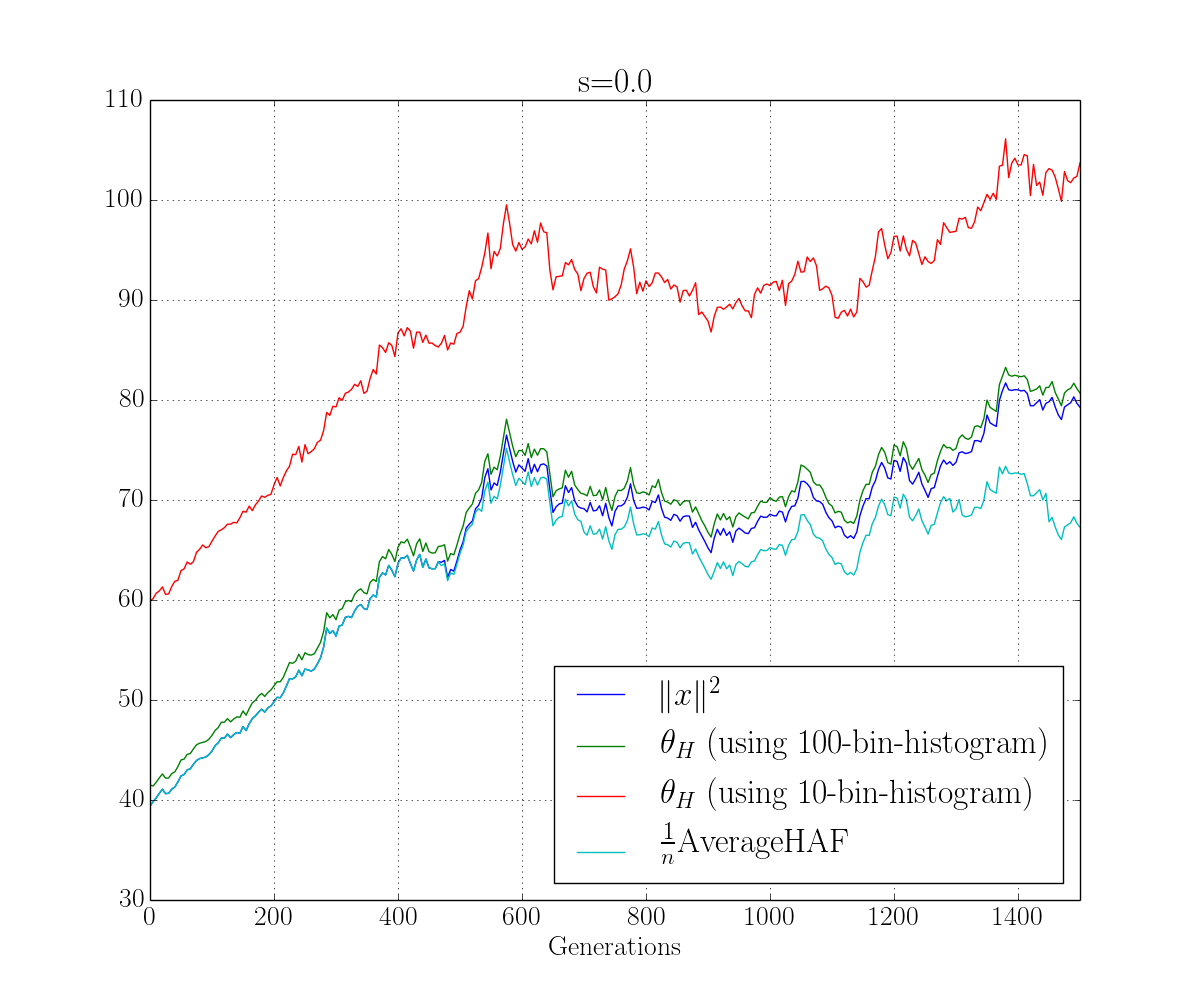
\includegraphics[scale=0.25]{thetaHs00} &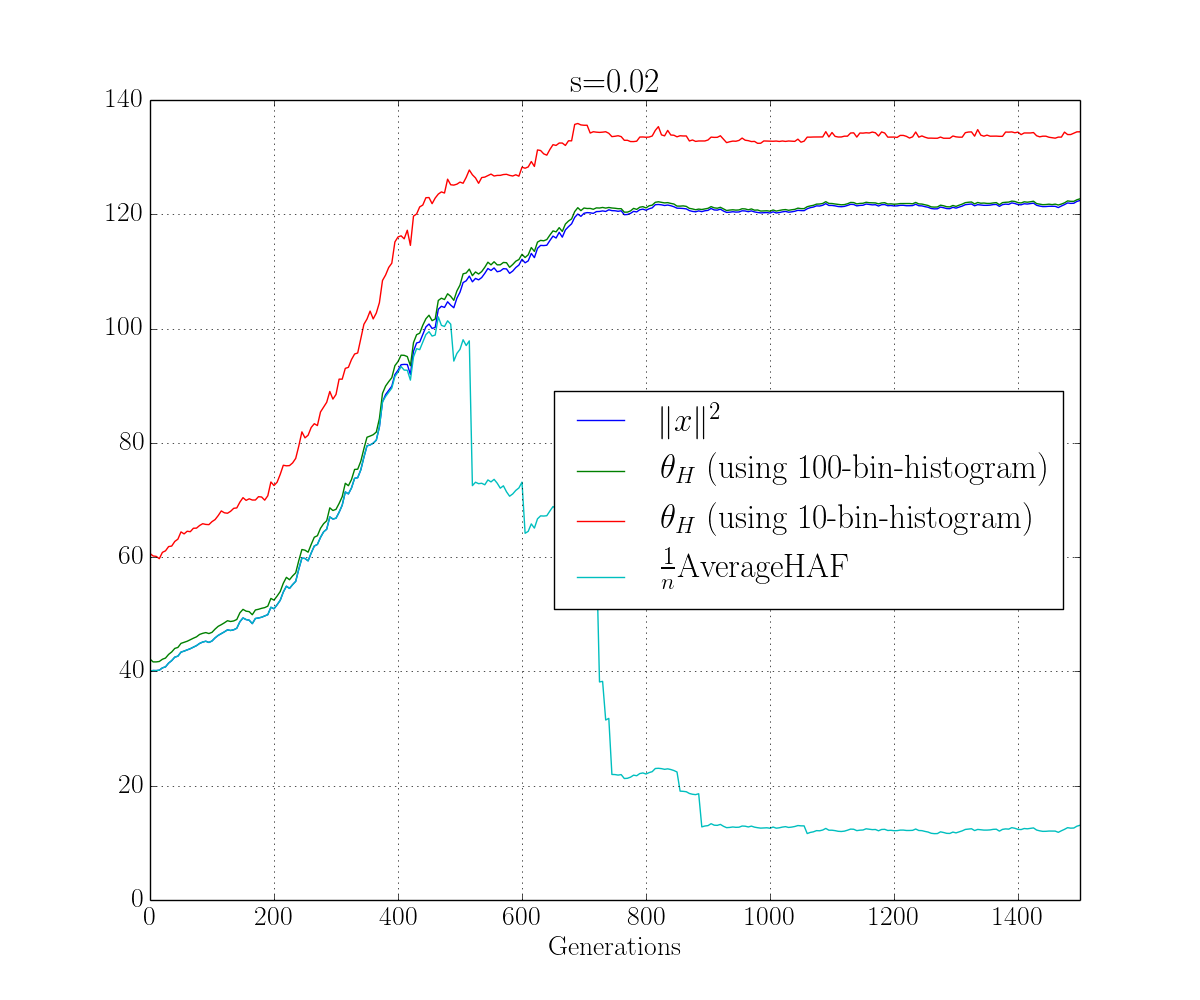
\includegraphics[scale=0.25]{thetaHs02}
\end{tabular}
\end{figure}

\subsection{Tajima's D}
We can compute Tajima's D in time as a function of $s$ and initial carrier frequency.

\beq
D_0&=\Pi_0 - W_0, \ \ \ \ \ D_t=\Pi_t - W_t\\
\Pi_t&= (1-\nu_t^2)\Pi_0 \\
W_0&= \frac{m_0}{S_n}, \ \ \ \ \ W_t= \frac{m_t}{S_n}\\
\frac{W_t}{W_0}&=\frac{\frac{m_t}{S}}{\frac{m_0}{S}} \ \ \Rightarrow W_t=\frac{m_t}{m_0}W0 \\
\frac{m_t}{m_0}&=\frac{\log\left((1-\nu_t)n +1 \right)}{\log(n)} \approx  \frac{\log\left((1-\nu_t)n\right)}{\log(n)} = \frac{\log(1-\nu_t)+\log(n)}{\log(n)} = 1+ \frac{ \log(1-\nu_t)}{\log(n)}\\
D_t&= (1-\nu_t^2)\Pi_0 - (1+ \frac{ \log(1-\nu_t)}{\log(n)} ) W_0 = D_0+\log(1-\nu_t) \frac{W_0}{\log(n)} -\nu_t^2 \Pi_0\\
\frac{d D_{t}}{d \nu_{t}}&=
 2\Pi_0\nu_t - \frac{\frac{W_0}{\log(n)}}{1-\nu_t}=a\nu_t + \frac{b}{1-\nu_t}
 \eeq

\subsection{Likelihood Ratio Test}
Using the MLE (and other) estimates of $s$ it is desirable to perform a secondary task such as \emph{testing for selection} or \emph{locating the site under selection}. Likelihood ratio test (LRT) statistics for time series \cite{feder2014} have shown to be predictors for differentiating neutral and natural selection evolution cases. For a single locus model, the likelihood ratio test statistics $\Lambda(s*)$ is defined
\beq \label{eq:lrt}
\Lambda(s^*) = \log \left(\frac{\Lc(\bfX|s=s*)}{\Lc(\bfX|s=0)}\right)
\eeq
where $s^*$ is the optimal solution for the maximum-likelihood procedure. For the Gaussian process and Gaussian model the likelihood $\Lc_{GP}$ and $\Lc_G$ are well defined and \eqref{eq:lrt} can be easily evaluated. The likelihood of the Naive method for estimating based on $x_t$ is 
\beq
\Lc_N(s|x_t,x_0)=x_t-\sigma(st/2 -c)
\eeq

In addition to LRT, the value of $s^*$ itself can be regarded as a signal for detecting selection. In other words, modifying the LRT to
\beq
\Theta=s^*\Lambda(s^*)
\eeq
will take into account of two different objectives, 1)model discrepancy from neutral model 2)strength of selection under non-neutral model. In the  results we show that the modified-LRT makes more accurate predictions.
\newpage
